\documentclass[letterpaper,10pt]{article}

\usepackage{enumitem}
\usepackage{titling}
\usepackage{listings,listings-rust}
\usepackage{url}
\usepackage{soul}
\usepackage{hyperref}
\usepackage{setspace}
\usepackage{subfig}
\usepackage{sectsty}
\usepackage{pdfpages}
\usepackage{colortbl}
\usepackage{multirow}
\usepackage{multicol}
\usepackage{relsize}
\usepackage{amsmath}
\usepackage{wasysym}
\usepackage{fancyvrb}
\usepackage[yyyymmdd]{datetime}
\usepackage{amsmath,amssymb,amsthm,graphicx,xspace}
\usepackage[titlenotnumbered,noend,noline]{algorithm2e}
\usepackage[compact]{titlesec}
\usepackage{XCharter}
\usepackage[T1]{fontenc}
\usepackage[scaled]{beramono}
\usepackage[normalem]{ulem}
\usepackage{booktabs}
\usepackage{tikz}
\usetikzlibrary{arrows.meta,automata,shapes,trees,matrix,chains,scopes,positioning,calc,decorations.pathreplacing}
\tikzstyle{block} = [rectangle, draw, fill=blue!20, 
    text width=2.5em, text centered, rounded corners, minimum height=2em]
\tikzstyle{bw} = [rectangle, draw, fill=blue!20, 
    text width=4em, text centered, rounded corners, minimum height=2em]

\definecolor{namerow}{cmyk}{.40,.40,.40,.40}
\definecolor{namecol}{cmyk}{.40,.40,.40,.40}
\renewcommand{\dateseparator}{-}

\let\LaTeXtitle\title
\renewcommand{\title}[1]{\LaTeXtitle{\textsf{#1}}}

\lstset{basicstyle=\footnotesize\ttfamily,breaklines=true}

\newcommand{\CPP}{C\nolinebreak\hspace{-.05em}\raisebox{.4ex}{\tiny\bf +}\nolinebreak\hspace{-.10em}\raisebox{.4ex}{\tiny\bf +}}
\def\CPP{{C\nolinebreak[4]\hspace{-.05em}\raisebox{.4ex}{\tiny\bf ++}}}

\newcommand{\handout}[5]{
  \noindent
  \begin{center}
  \framebox{
    \vbox{
      \hbox to 5.78in { {\bf ECE459: Programming for Performance } \hfill #2 }
      \vspace{4mm}
      \hbox to 5.78in { {\Large \hfill #4  \hfill} }
      \vspace{2mm}
      \hbox to 5.78in { {\em #3 \hfill \today} }
    }
  }
  \end{center}
  \vspace*{4mm}
}

\newcommand{\lecture}[3]{\handout{#1}{#2}{#3}{Lecture#1}}
\newcommand{\tuple}[1]{\ensuremath{\left\langle #1 \right\rangle}\xspace}

\addtolength{\oddsidemargin}{-1.000in}
\addtolength{\evensidemargin}{-0.500in}
\addtolength{\textwidth}{2.0in}
\addtolength{\topmargin}{-1.000in}
\addtolength{\textheight}{1.75in}
\addtolength{\parskip}{\baselineskip}
\setlength{\parindent}{0in}
\renewcommand{\baselinestretch}{1.5}
\newcommand{\term}{Winter 2020}

\singlespace


\begin{document}

\lecture{23 --- Password Cracking, Software Transactional Memory}{\term}{Patrick Lam \& Jeff Zarnett}

\section*{GPU Application: Password Cracking}

GPUs are good---too good, even---at password cracking. We'll discuss a paper
that proposes a technique to make it harder to crack passwords. This technique
is scrypt, the algorithm behind DogeCoin~\cite{scrypt}. See also \url{http://www.tarsnap.com/scrypt.html}

First, let's talk about acceptable practices for password storage. It is \emph{not}
acceptable engineering practice to store passwords in plaintext. The inevitable security
breach will end with your company sending a ``sorry'' disclosure email to its clients,
and you will be responsible for the ensuing bad publicity.

Acceptable practices: {\bf not} plaintext; hashed and salted.
(We're not going to talk about what ``salted'' means here. Look it up if you need it. Hint: ECE 155.)

\paragraph{Cryptographic hashing.} Instead of storing the plaintext password, you
store a hash of the password, under a cryptographic hash function. One important
property of a cryptographic hash function is that it must be (believed to be a) one-way
function; that is: $x \mapsto f(x)$, the forward direction, must be easy to compute, but
$f(x) \mapsto x$, the inverse mapping, must be hard to compute. Examples of such functions
include SHA1 and scrypt.

\paragraph{Breaking the hash.} Even if there is no known short computation for the
inverse function, it's always possible to brute-force the password
computation by trying all possible passwords. Think about how GPUs
work. Each potential password is a point in the computation space, and
we compute the hash over all of them simultaneously.  That's a lot of
speedup. Custom hardware is also good, and those of you who know
something about hardware could think about implementing
it. Oh, hello, Bitcoin miners. 

\paragraph{Arms race: making cracking difficult.} The idea has always been
to make it more difficult to compute the hash function, so that it's OK to
try one password, but it's intractable to try one billion passwords. Even way back,
UNIX passwords forced repeated applications of the hash function to accomplish these.

The main idea behind scrypt is to make hashing expensive in both time and space,
increasing both the number of operations and the cost of brute-forcing.
Hence crackers will need to use more circuitry to break passwords.

Of course, there's always this form of cracking:
\begin{center}
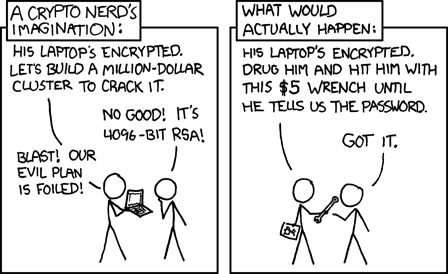
\includegraphics[width=0.5\textwidth]{images/xkcd-538}\\
\hfill (Source: xkcd 538)
\end{center}

\newtheorem{defn}{Definition}

\paragraph{Formalization.} Let's make the notion of ``expensive'' a bit more formal.
The idea is to force the use of the ``most memory possible'' for a given number of
operations. More memory implies more circuitry required to implement.

    \begin{defn}
      A \emph{memory-hard} algorithm on a Random Access Machine is an
      algorithm which uses $S(n)$ space and $T(n)$ operations, where
      $S(n) \in \Omega(T(n)^{1-\varepsilon})$.
    \end{defn}

Memory-hard algorithms are expensive to implement in either hardware or software.

Now, we want to move from particular algorithms to the underlying
functions (that is, we would like to quantify over all possible
algorithms). Intuitively, a \emph{sequential memory-hard function} is
one where (1) the fastest sequential algorithm is memory-hard; and (2)
it is impossible for a parallel algorithm to asymptotically achieve
lower cost.

\paragraph{Existence proof.} Of course anyone can define anything.
It's much better if the thing being defined actually exists. The
scrypt paper then goes on to exhibit ReMix, which is a concrete
example of a sequential memory hard function.

Finally, the paper concludes with an example of a more realistic
(cache-aware) model and a hard function in that context, BlockMix.

\section*{Reduced-resource computation}
In an n-body simulation, you can implement an optimization that
trades off accuracy for performance. In that specific case, 
domain knowledge would enable you to skimp out on
some unnecessary computation: points that are far away contribute only
very small forces.

In~\cite{Rinard:2010:PSA:1932682.1869525}, Martin Rinard summarizes
two of his novel ideas for automatic or semiautomatic optimizations
which trade accuracy for performance: early phase
termination~\cite{Rinard:2007:EarlyPhaseTermination} and loop
perforation~\cite{hoffmann09:_using_code_perfor_improv_perfor}. Both
of these ideas are applicable to code we've learned about in this
class.

\subsection*{Early phase termination}
We've talked about barriers quite a bit. Recall that the idea is that
no thread may proceed past a barrier until all of the threads
reach the barrier. Waiting for other threads causes delays. 
Killing slow threads obviously speeds up the program. Well, that's easy.

\begin{center}
``Oh no, that's going to change the meaning of the program!''
\end{center}

Let's consider some arguments about when it may be acceptable to just
kill (discard) tasks. Since we're not completely crazy, we can develop
a statistical model of the program behaviour, and make sure that the
tasks we kill don't introduce unacceptable distortions. Then when we
run the program, we get an output and a confidence interval.

\paragraph{Two Examples.} When might this work? Monte Carlo simulations
are a good candidate; you're already picking points randomly.
Raytracers can work as well. Both of these examples could spawn a lot
of threads and wait for all threads to complete.  In either case, you
can compensate for missing data points, assuming that they look like
the ones that you did compute.

Also recall that, in scientific computations, you're entering points
that were measured (with some error) and that you're computing
using machine numbers (also with some error). Computers are only
providing simulations, not the ground truth; the question is
whether the simulation is good enough.

\subsection*{Loop perforation} 
You can also apply the same idea to sequential programs. Instead
of discarding tasks, the idea here is to discard loop iterations.
Here's a simple example: instead of the loop,
\begin{center}
\verb|for (i = 0; i < n; i++) sum += numbers[i];|
\end{center} \vspace*{-1em}
simply write,
\vspace*{-1em}\begin{center}
\verb|for (i = 0; i < n; i += 2) sum += numbers[i];|
\end{center}
and multiply the end result by a factor of 2. This only works 
if the inputs are appropriately distributed, but it does give a
factor 2 speedup.

\paragraph{Example domains.} In~\cite{Rinard:2010:PSA:1932682.1869525},
we can read that loop perforation works for evaluating forces on water
molecules (in particular, summing numbers); Monte-Carlo simulation for
swaption pricing; and video encoding. In that example, changing loop
increments from 4 to 8 gives a speedup of 1.67, a signal to noise ratio
decrease of $0.87\%$, and a bitrate increase of $18.47\%$, producing
visually indistinguishable results. The computation looks like this:

{\small
\begin{verbatim}
min = DBL_MAX;
index = 0;
for (i = 0; i < m; i++) {
  sum = 0;
  for (j = 0; j < n; j++) sum += numbers[i][j];
  if (min < sum) {
    min = sum;
    index = i;
  }
}
\end{verbatim}
}
The optimization changes the loop increments and then compensates. 

\section*{Software Transactional Memory}
Developers use software transactions by 
writing {\tt atomic} blocks. These blocks are just like {\tt
  synchronized} blocks, but with different semantics.

\begin{lstlisting}
  atomic {
    this.x = this.z + 4;
  }
\end{lstlisting}
You're meant to think of database transactions, which I expect you to
know about. The {\tt atomic} construct means that either the code in
the atomic block executes completely, or aborts/rolls back in the
event of a conflict with another transaction (which triggers a retry
later on).

\paragraph{Benefit.} The big win from transactional memory is the simple
programming model. It is far easier to program with transactions than with
locks. Just stick everything in an atomic block and hope the compiler does the
right thing with respect to optimizing the code.

\paragraph{Motivating Example.} We'll illustrate STM with the usual bank account example\footnote{Apparently, bank account transactions aren't actually atomic, but they still make a good example.}.
  \begin{lstlisting}
transfer_funds(Account* sender, Account* receiver, double amount) {
  atomic {
    sender->funds -= amount;
    receiver->funds += amount;
  }
}
  \end{lstlisting}

Using locks, we have two main options:
      \begin{itemize}
        \item Big Global Lock: Lock everything to do with modifying accounts. (This is slow; and you might forget to grab the lock).
        \item Use a different lock for every account. (Prone to deadlocks; may forget to grab the lock).
      \end{itemize}
With STM, we do not have to worry about remembering to acquire locks,
or about deadlocks.

\paragraph{Drawbacks.} As I understand it, three of the problems with 
transactions are as follows:

\begin{itemize}
\item I/O: Rollback is key. The problem with transactions and I/O is
  not really possible to rollback. (How do you rollback a write to the
  screen, or to the network?)

\item Nested transactions: The concept of nesting transactions is easy
  to understand. The problem is: what do you do when you commit the
  inner transaction but abort the nested transaction? The clean
  transactional fa\,cade doesn't work anymore in the presence of
  nested transactions.

\item Transaction size: Some transaction implementations (like
  all-hardware implementations) have size limits for their
  transactions.
\end{itemize}

\paragraph{Implementations.} Transaction implementations are typically 
optimistic; they assume that the transaction is going to succeed,
buffering the changes that they are carrying out, and rolling back the
changes if necessary.

One way of implementing transactions is by using hardware support,
especially the cache hardware. Briefly, you use the caches to store
changes that haven't yet been committed. Hardware-only transaction
implementations often have maximum-transaction-size limits, which are
bad for programmability, and combining hardware and software approaches
can help avoid that.

\paragraph{Implementation issues.} Since atomic sections don't protect
against data races, but just rollback to recover, a datarace may still
trigger problems in your program.

\begin{tabular}{r|l}
\hspace*{2em}  \begin{minipage}{.4\textwidth}
\begin{lstlisting}
atomic {
  x++;
  y++;
}
\end{lstlisting}
\end{minipage}
&
\hspace*{2em} \begin{minipage}{.4\textwidth}
\begin{lstlisting}
atomic {
  if (x != y)
     while (true) { }
}
\end{lstlisting}
\end{minipage}
\end{tabular}

In this silly example, assume initially {\tt x = y}. You may think the
code will not go into an infinite loop, but it can.

\bibliographystyle{alphaurl}
\bibliography{459}


\end{document}
